\chapter{Zásuvný modul}
\label{4-plugin}

Čtvrtá kapitola popisuje vývoj zásuvného modulu a~rozebírá důležité části kódu. 

\section{Obsah CSV}
\label{obsah}

Vstupní soubor s~měřenými daty musí být tzv.~\zk{CSV}~(\textit{comma-separated values} - hodnoty oddělené
čárkami) soubor. Oddělování čárkami představuje pro čtení souboru zásuvným modulem zásadní podmínku.
Software v~měření radioaktivity (a~mnohdy i~jiných atributů) běžně používaný k~zápisu obvykle
produkuje právě soubory s~koncovkou~.\zk{CSV} a~s~nezbytnými i~doplňujícími atributy. Na pořadí
atributů nezáleží. 

Povinné části a~jejich označení v~hlavičce souboru: 
\begin{itemize}

	\item RECS: Pod označením RECS se skrývá číslo bodu. Tato položka je nezbytná pouze
	v~případě \textit{posunu o~hodnoty} (kvůli přepisu označení bodu z~důvodu zachování úzu číslování
	od čísla~0). Avšak číslování bodů zajišťuje čitelnost dat, pročež je silně doporučováno vždy. 
	
	\item Lat\_deg: Lat\_deg označuje sloupec obsahující zeměpisnou šířku snímaného bodu na elipsoidu.
	Za referenční elipsoid, na němž se úloha vypočítává, byl zvolen nejběžněji užívaný
	elipsoid~\zk{WGS84}. 
	
	\item Lon\_deg: Lon\_deg označuje sloupec obsahující zeměpisnou délku snímaného bodu na elipsoidu.
	Za referenční elipsoid, na němž se úloha vypočítává, byl zvolen nejběžněji užívaný
	elipsoid~\zk{WGS84}. 
	
	\item mereni: mereni obsahuje měřenou hodnotu (v~prezentovaném případě hodnotu radioaktivity, ale
	sloupec by mohl obsahovat jakoukoli jinou, i~nečíselnou hodnotu). 
	
	\item Gtm\_sec: Čas měření ve vteřinách. Není důležité, jaký typ udávání času daný soubor
	podporuje (zda například počítá vteřiny od nějakého roku, nebo od začátku měření), počítá
	se s~rozestupy mezi jednotlivými údaji. 

\end{itemize}

Soubor bývá doplněn o~data pro zásuvný modul zbytná, například číslo linie, souřadnice na jiném
referenčním tělese, nadmořskou výšku, jiný systém času nebo datace. 

  \begin{figure}[H]
   \centering
	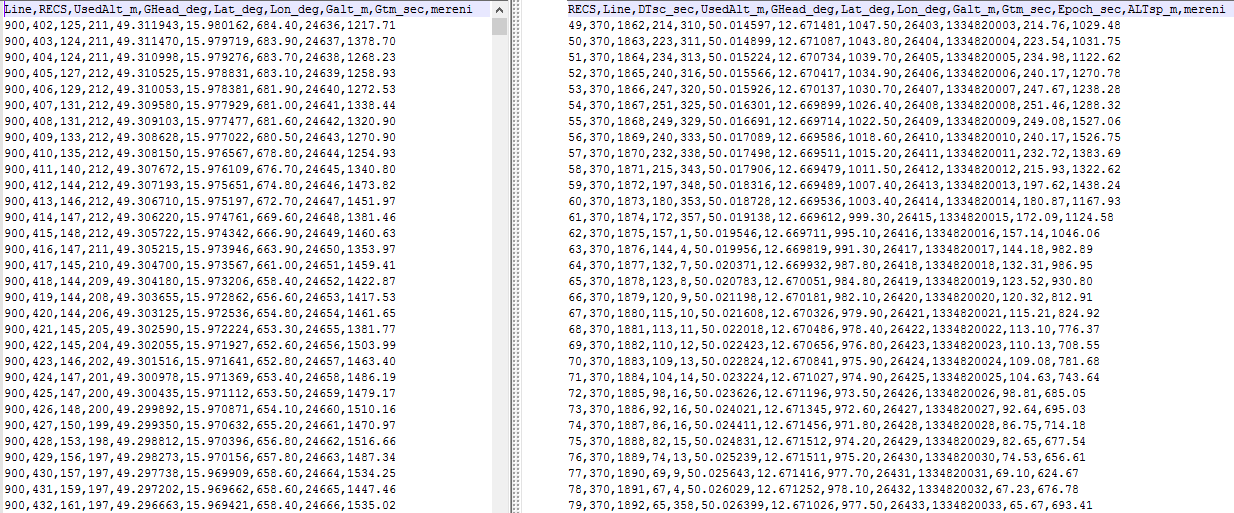
\includegraphics[scale=0.45]{./pictures/ukazka-vstup.png}
	\caption[Ukázka dvou typů vstupních souborů]{Ukázka dvou typů vstupních souborů
      \label{fig:ukazka-vstup}}
  \end{figure}

\section{Tělo zásuvného modulu}
\label{telo}

Kosmogonický základ zásuvného modulu byl vytvořen ve volně šiřitelném mo\-dulu nazvaném Plugin
Builder\footnote{Dostupný na \textit{https://plugins.qgis.org/plugins/pluginbuilder/}}. Jedná se
o~zásuvný modul vytvořený pro QGIS především (ale nikoli pouze) suitou kolem GeoApt LLC (například Gary
Sherman), skupi\-ny zaměřující se na volný \zk{GIS}. Plugin Builder na
základě uživatelem zadaných parametrů vytvoří základní skelet zásuvného modulu - tlačítko, holobyt
grafického rozhraní, metadata, základní funkce (zapnout, vypnout) a~vazby zásuvného modulu. 

Fundamentální tělo zajišťující základní funkcionalitu zásuvného modulu je ulože\-no v~několika vzájemně
provázaných souborech: 
\begin{itemize}

	\item \_\_init\_\_.py: Základní inicializace zásuvného modulu. 

	\item plugin\_upload.py: Zajišťuje všeobecnou dostupnost zásuvného modulu. 	

	\item suro\_leveling.py: Implementuje zásuvný modul do prostředí QGIS. Načítá jeho ikonu,
	jmenuje a~aktivuje jej a~v~případě vypínání se stará o~jeho destrukci. Funkce \textit{run} jej váže se
	suro\_leveling\_dockwidget.py. 
	
	\item suro\_leveling\_dockwidget.py: Nejdůležitější ze základních souborů. Zde se přes volání
	\textit{.ui} souboru suro\_leveling\_dockwidget\_base.ui vytvořeného v~prostředí Qt Designer
	vyvolává grafické uživatelské rozhraní. Zajišťuje také funkčnost ve\-škerých jeho částí, od načítání
	cest vstupních a~výstupních dat přes jejich zobrazování (volá show\_as\_layer.py) až po samotné volání
	posunu (move.py). Na pozadí dochází ke kontrole vstupujících údajů, v~případě nesrovnalostí
	bude uživatel upozorněn chybovým hlášením. Aby se zamezilo zbrklým nehodám, byl ke zpřístupnění
	tlačítek zabudován hlídací pes - ke zpřístupnění tlačítka na zobrazení vstupního souboru musí být
	k~tomuto souboru definována cesta, taktéž k samotnému posunu je třeba mít vyplněny všechny potřebné
	parametry. 
	
	\item show\_as\_layer.py: Zobrazí soubor, an je předán jako jeden ze vstupních parame\-trů. Druhým
	vstupním parametrem je styl, jenž bude při zobrazování použit. Aby se zamezilo graviditě kódu
	a~obecné duplicitě kódu v~podhoubí prostředí QGIS, byly k~zobrazení využity interní objekty
	QgsVectorLayer a~QgsMapLayerRegistry. 

\end{itemize}

Toliko k~hrubému náčrtu fungování zásuvného modulu. Některé dílčí složky byly při představování
zane\-dbány, poněvadž nejsou k~pochopení fungování mo\-dulu nezbytné. Nyní se zvlášť podívejme na
soubory související se zkoumanou pro\-blematikou, tedy obsah move.py. 

\section{Posun o hodnoty}
\label{by_points}

Posun o~hodnoty se skrývá pod funkcí move.by\_points. Zde nejprve proběhne analýza vstupních dat.
Analýza spočívá v~prohledání hlavičky souboru, je třeba zjistit polohu hledaných hodnot - sloupec
\textit{mereni}. Veškeré hodnoty z~tohoto sloupce uloží jako seznam měření. 

Následně se čte vstupní soubor řádek po řádku a~postup posunu se liší na základě vstupní hodnoty posunu. 

Jedná-li se o~číslo kladné, v~každé smyčce cyklu se ze seznamu měření odejme hodnota na pozici
voleného posunu a~uloží (cyklus probíhá do té doby, dokud na dané pozici existuje nějaký prvek). Do paměti
počítače se přečte řádek vstupního souboru a~hodnota ve sloupci \textit{mereni} se přepíše vyňatým prvkem. 
Následně se modifikovaný řádek zapíše do výstupního souboru. 

Jedná-li se o~číslo záporné, ještě před cyklem se provede odečtení X~řádků bez zápisu, kde X je hodnota
posunu. Následně probíhá syžet tímtéž způsobem s~tím rozdílem, že se navíc k~hodnotě ve sloupci
\textit{RECS}, tedy číslu bodu, přičítá hodnota posunu (záporná hodnota, tudíž se číslo bodu
zmenšuje). Tento krok není pro posun nikterak zásadní, alebrž slouží pouze k~dodržení úzu - body
se číslují od numera~0. 

Ve speciálním případě, kdy vstupuje do posunu o~hodnoty číslice~0, dochází k~pouhému kopírování vstupního
souboru do souboru výstupního. Ovšem na žádný pád nemá v~takovém případě použití zásuvného modulu
odůvodnění. 

\section{Posun o konstantní vzdálenost}
\label{by_distance}

\subsection{Výpočet azimutu}
\label{azimut}

\subsection{První geodetická úloha}
\label{prvniguplugin}

\section{Posun o konstantní čas (proměnnou vzdálenost)}
\label{by_seconds}

\section{Licence}
\label{licence}

Nebtě byl zásuvný modul vytvořen pro QGIS a~využívá jeho knihoven, dědí jeho licenci: GNU General Public
License (\zk{GPL}). 



